\section{Results}
\label{sec:results}

\newcommand{\pairsN}{3,950}
\newcommand{\pairsMoved}{29.9}
\newcommand{\pairsUp}{638}
\newcommand{\pairsDown}{543}

\newcommand{\cfRuns}{1,189}
\newcommand{\cfRend}{4,756}
\newcommand{\cfMediumMovedTest}{48.6}
\newcommand{\cfMediumMovedOod}{74.2}
\newcommand{\cfFetchMovedTest}{20.4}
\newcommand{\cfFetchMovedOod}{18.8}


We report Job pods first, because they are the plain Kubernetes case, with no orchestrator to absorb mistakes.
Flyte pods follow, and so does the comparison between the two. Numbers are regret in percent against the cheapest
request, seed 1, with 95\% intervals clustered by task, unless noted.

\subsection{Leaderboard}
\label{sec:res-lead}

\Cref{tab:leaderboard,fig:tradeoff} give the main results. On new tasks from familiar families, the trees pooled
with the decision model are best at \rTestPoolDec\% \ciTestPoolDec. The trees pooled with the RL model and read by
argmax (\rTestPoolRLArg\%) cannot be separated from it (paired difference \vbTestPoolRLArg\ points
\vbTestPoolRLArgCI). The gate (\rTestGate\%) and RL read by argmax (\rTestRLArg\%) are about two points behind.
All four are ahead of the trees alone (\rTestTrees\%) and the decision model alone (\rTestDec\%), and far ahead of
the rules (\rTestSized\% for rules-sized, \rTestRules\% for rules) and the zero-shot model (\rTestZS\%). A static
request costs about twice the cheapest one.

On the seven held-out families every approach does worse, and the order changes. Rules-sized (\rUnseenSized\%) and
the gate (\rUnseenGate\%) have the lowest regret, and the gate equals the decoded RL model it routes those pods to.
The read-outs validation chose for the trained models do worse: RL read by argmax reaches \rUnseenRLArg\%, the
decision model \rUnseenDec\%, the pools \rUnseenPoolDec--\rUnseenPoolRLArg\%, and the trees \rUnseenTrees\%. The
zero-shot model is at \rUnseenZS\% on its smaller sample. Clustered by family, the intervals on this split are
wide: rules-sized spans \ciFamUnseenSized\ and RL read by argmax \ciFamUnseenRLArg, and of the approaches in
\cref{tab:leaderboard} only the static request is clearly worse than rules-sized.

\begin{table}[tbp]
\centering\small
\caption{Regret (\%) on Job pods for seed 1, with 95\% intervals clustered by task, and for the unseen split also
by family; regret on Flyte pods; dollar regret on Job pods; and the mean and range of Job regret over three
trainings. Each trained model is shown with the read-out validation chose (\cref{tab:readouts}). Bold marks the
approaches whose paired difference from the column's best includes zero. Each split has 5,095 Job pods for test
and 6,416 for unseen. $^\dagger$Zero-shot is scored on a sample of 130 test and 150 unseen Job pods
(\cref{tab:zs}) and is not compared for bold.}
\label{tab:leaderboard}
\resizebox{\linewidth}{!}{\begin{tabular}{@{}lrrrrrrrr@{}}
\toprule
& \multicolumn{2}{c}{Job pods: regret (\%)} & \multicolumn{2}{c}{Flyte pods} & \multicolumn{2}{c}{Job \$ regret} & \multicolumn{2}{c}{Job, 3 seeds: mean (range)} \\
\cmidrule(lr){2-3}\cmidrule(lr){4-5}\cmidrule(lr){6-7}\cmidrule(l){8-9}
approach & test & unseen & test & unseen & test & unseen & test & unseen \\
\midrule
static & 89.3\,{\scriptsize[84.7, 93.7]} & 115.1\,{\scriptsize[111.2, 119.2]} & 91.5 & 112.8 & 183.0 & 258.1 & 89.3 & 115.1 \\
rules & 42.4\,{\scriptsize[37.9, 46.7]} & 49.8\,{\scriptsize[47.0, 52.5]} & 41.3 & 48.0 & 56.9 & 120.3 & 42.4 & 49.8 \\
rules-sized & 37.7\,{\scriptsize[33.8, 41.6]} & \textbf{39.2}\,{\scriptsize[37.3, 41.2]} & 37.3 & 41.1 & 55.9 & 117.9 & 37.7 & 39.2 \\
zero-shot 27B & 48.8\,{\scriptsize[33.1, 67.2]} & 42.8\,{\scriptsize[29.6, 57.2]} & 35.7 & 52.0 & 86.0 & 30.0 & --- & --- \\
zero-shot 27B, JSON & 48.8\,{\scriptsize[31.9, 67.7]} & 44.4\,{\scriptsize[31.2, 59.2]} & 21.8 & 51.5 & 100.8 & 81.9 & --- & --- \\
trees & 11.5\,{\scriptsize[10.2, 12.8]} & 69.1\,{\scriptsize[66.3, 71.8]} & 14.6 & 69.0 & 30.6 & \textbf{85.6} & 11.5 & 69.1 \\
decision & 12.6\,{\scriptsize[11.3, 14.0]} & 47.8\,{\scriptsize[45.6, 50.4]} & 11.3 & 43.0 & 39.6 & 119.0 & 13.7\,{\scriptsize(12.6--15.0)} & 49.5\,{\scriptsize(44.2--56.6)} \\
decision, argmax & 30.3\,{\scriptsize[28.0, 32.5]} & 69.1\,{\scriptsize[66.2, 72.1]} & 28.7 & 63.8 & 39.8 & 107.2 & 30.8\,{\scriptsize(30.3--31.7)} & 72.6\,{\scriptsize(68.1--80.6)} \\
RL & 14.6\,{\scriptsize[13.2, 16.1]} & 39.3\,{\scriptsize[37.3, 41.4]} & 14.3 & \textbf{40.2} & 50.6 & 127.9 & 16.2\,{\scriptsize(14.6--17.4)} & 37.7\,{\scriptsize(35.5--39.3)} \\
RL, argmax & 8.5\,{\scriptsize[7.1, 9.9]} & 46.5\,{\scriptsize[44.2, 48.8]} & 8.6 & 46.2 & 35.3 & 106.4 & 8.4\,{\scriptsize(8.2--8.6)} & 45.0\,{\scriptsize(41.3--47.2)} \\
pool $\times$ decision & \textbf{6.6}\,{\scriptsize[5.6, 7.6]} & 56.8\,{\scriptsize[54.5, 59.2]} & \textbf{5.5} & 51.4 & 27.6 & 95.0 & 6.8\,{\scriptsize(6.6--6.9)} & 55.7\,{\scriptsize(52.1--58.3)} \\
pool $\times$ RL & 10.5\,{\scriptsize[9.4, 11.8]} & 49.6\,{\scriptsize[47.5, 51.8]} & 11.1 & 50.3 & 34.7 & 100.8 & 10.7\,{\scriptsize(10.5--11.0)} & 53.9\,{\scriptsize(49.6--61.3)} \\
pool $\times$ RL, argmax & 7.2\,{\scriptsize[6.0, 8.4]} & 79.4\,{\scriptsize[75.7, 83.2]} & 7.1 & 78.1 & \textbf{15.7} & 111.6 & 8.6\,{\scriptsize(6.8--11.8)} & 89.6\,{\scriptsize(78.6--110.9)} \\
gate (kNN, $q$ 0.95) & 8.1\,{\scriptsize[6.9, 9.4]} & 39.3\,{\scriptsize[37.3, 41.4]} & 7.6 & \textbf{40.2} & 19.5 & 127.9 & 9.6\,{\scriptsize(8.1--12.7)} & 37.7\,{\scriptsize(35.5--39.3)} \\
\bottomrule
\end{tabular}
}
\end{table}

\begin{figure}[tbp]
\centering
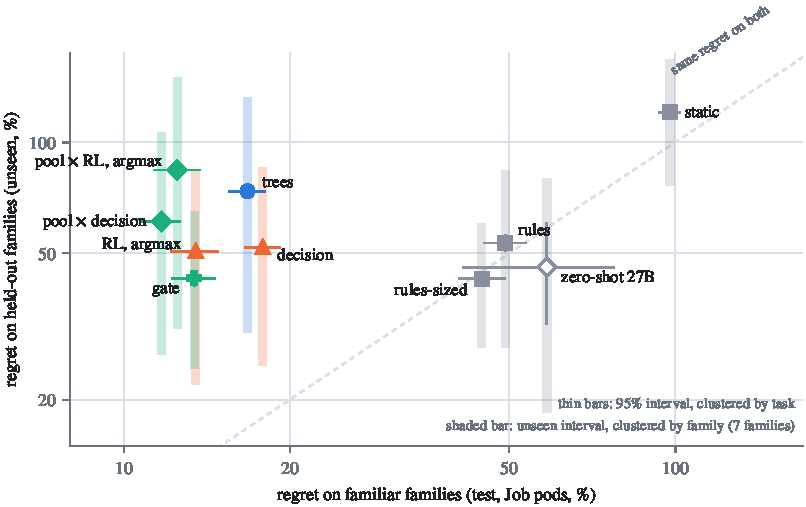
\includegraphics[width=\linewidth]{figures/fig_tradeoff.pdf}
\caption{Regret on familiar families against regret on held-out families, Job pods, seed 1 (log scales). Gray:
static request, rules and zero-shot (hollow: scored on a sample). Blue: trees. Orange: language models. Green:
pools and the gate. No approach is in the lower left: the approaches that lead on familiar code fall behind a
sized rule on new code.}
\label{fig:tradeoff}
\end{figure}

The gate is the only trained approach near the top on both splits, at a cost of
\diffTestGatePoolRLArg\ points on familiar code \diffTestGatePoolRLArgCI\ against its familiar-code member and a
saving of \diffUnseenGatePoolRLArg\ points on new code \diffUnseenGatePoolRLArgCI. It does not beat rules-sized on
new code (\diffUnseenSizedGate\ points \diffUnseenSizedGateCI), and its members were chosen with the same held-out
families in view (\cref{sec:res-gate}).

\subsection{Seen code, new programs and new families}
\label{sec:res-code}

Most familiar-family test tasks are programs the models have seen. \codeSeenShare\% of test Job pods run code
identical to a training task's, and differ only in input sizes and history. \Cref{tab:code} splits the test split
in two. On the \codeNovelN{} pods with new programs, regret rises for every trained approach. The decision model
goes from \seenDec\% to \novelDec\%. The trees pooled with the RL model and read by argmax barely move
(\seenPoolRLArg\% to \novelPoolRLArg\%), and the gate goes from \seenGate\% to \novelGate\%. The held-out families
are the larger step: new programs from familiar families stay within 13--35\% of the cheapest request, while every approach is at about 43\% or worse on the new
families. Rules-sized reads only sizes and the pod spec, so it is the same on both halves.

\begin{table}[tbp]
\centering\small
\caption{Job regret (\%) on test pods whose task code appears in training (seen) and on those whose code does
not (new), with the unseen families for comparison, for seed 1.}
\label{tab:code}
\begin{tabular}{@{}lrrr@{}}
\toprule
& \multicolumn{2}{c}{test: code in training?} & \\
\cmidrule(lr){2-3}
approach & seen (4,135) & new (960) & unseen families \\
\midrule
static & 86.1 & 148.0 & 120.7 \\
rules & 52.0 & 36.7 & 53.3 \\
rules-sized & 44.5 & 44.4 & 42.7 \\
trees & 15.7 & 21.4 & 73.8 \\
decision & 14.0 & 34.3 & 51.9 \\
RL, argmax & 11.6 & 21.8 & 50.6 \\
pool $\times$ decision & 10.3 & 17.9 & 61.0 \\
pool $\times$ RL, argmax & 12.4 & 13.2 & 84.1 \\
gate & 12.6 & 16.8 & 42.8 \\
\bottomrule
\end{tabular}

\end{table}

Part of the gap between test and unseen comes from the corpus mix: GPU runs are 36\% of unseen pods and 22\% of
test pods. \Cref{tab:corpus} in \cref{app:extra} breaks results down by corpus. The trees' weakness on new code is
concentrated in CPU and GPU families (\cUnseenCpuTrees\% and \cUnseenGpuTrees\%), and rules-sized is strongest on the
held-out CPU families (\cUnseenCpuSized\%).

\subsection{Does a model need to see Jobs?}
\label{sec:res-training}

\Cref{tab:training} trains the trees, the decision model and the pool three ways: on both pod types, on Jobs alone,
and on Flyte tasks alone. Flyte data does not make the models better on Jobs. A decision model trained only on Jobs
scores \rTestDecJob\% on Job test pods, against \rTestDec\% for one trained on both, a difference of
\diffTestDecDecJob\ points \diffTestDecDecJobCI; on seed 3 the Job-only model is better. The trees and the pool
behave the same way. The reverse transfer does not work. A model trained only on Flyte tasks scores \rTestDecFlyte\%
on Job pods, and the pool built on it reaches \rTestPoolDecFlyte\% where the pool trained on both reaches
\rTestPoolDec\%. A model trained only on Jobs also does worse on Flyte pods (\rFTestDecJob\% against \rFTestDec\%),
by less, because a Flyte task is closer to a Job with a small fixed runtime added than the other way around. On the
unseen families, the model trained on both pod types is ahead by \diffUnseenDecDecJob\ points
\diffUnseenDecDecJobCI, which may reflect the larger number of distinct workloads it saw.

\begin{table}[tbp]
\centering\small
\caption{What the training data includes. Regret (\%) on Job and Flyte pods, and the share of Job pods whose first
attempt succeeds, for seed 1.}
\label{tab:training}
\begin{tabular}{@{}llrrrrr@{}}
\toprule
&& \multicolumn{2}{c}{Job pods: regret (\%)} & \multicolumn{2}{c}{Flyte pods: regret (\%)} & Job \\
\cmidrule(lr){3-4}\cmidrule(lr){5-6}
approach & trained on & test & unseen & test & unseen & first OK \\
\midrule
trees & both & 11.5\,{\scriptsize[10.2, 12.8]} & 69.1 & 14.6\,{\scriptsize[13.3, 16.1]} & 69.0 & 97.6 \\
 & Jobs only & 11.8\,{\scriptsize[10.5, 13.1]} & 68.6 & 26.2\,{\scriptsize[24.4, 28.0]} & 78.9 & 97.7 \\
 & Flyte only & 18.3\,{\scriptsize[16.8, 19.9]} & 73.5 & 15.9\,{\scriptsize[14.5, 17.3]} & 93.5 & 94.1 \\
\midrule
decision & both & 12.6\,{\scriptsize[11.3, 14.0]} & 47.8 & 11.3\,{\scriptsize[10.0, 12.6]} & 43.0 & 97.2 \\
 & Jobs only & 13.2\,{\scriptsize[11.8, 14.7]} & 56.1 & 20.5\,{\scriptsize[18.8, 22.3]} & 53.6 & 97.0 \\
 & Flyte only & 37.3\,{\scriptsize[35.1, 39.6]} & 59.0 & 12.0\,{\scriptsize[10.6, 13.5]} & 48.5 & 87.2 \\
\midrule
decision, argmax & both & 30.3\,{\scriptsize[28.0, 32.5]} & 69.1 & 28.7\,{\scriptsize[26.5, 31.0]} & 63.8 & 87.3 \\
 & Jobs only & 28.8\,{\scriptsize[26.7, 31.1]} & 74.4 & 41.4\,{\scriptsize[38.8, 44.0]} & 79.3 & 87.0 \\
 & Flyte only & 56.2\,{\scriptsize[53.3, 59.3]} & 84.4 & 27.5\,{\scriptsize[25.4, 29.6]} & 66.6 & 76.9 \\
\midrule
pool $\times$ decision & both & 6.6\,{\scriptsize[5.6, 7.6]} & 56.8 & 5.5\,{\scriptsize[4.6, 6.6]} & 51.4 & 98.3 \\
 & Jobs only & 7.7\,{\scriptsize[6.6, 8.8]} & 57.9 & 17.1\,{\scriptsize[15.6, 18.6]} & 58.7 & 98.0 \\
 & Flyte only & 24.8\,{\scriptsize[22.9, 26.7]} & 51.6 & 5.4\,{\scriptsize[4.4, 6.5]} & 49.6 & 91.3 \\
\bottomrule
\end{tabular}

\end{table}

A model trained on both pod types treats them almost the same. The paired difference between a run's Job pod and
its Flyte pod is under two points on familiar code for every language model and pool (\cref{tab:gap}), and for the
RL model it is indistinguishable from zero; the trees do 3.0 points better on Jobs. On new code, the decision model and
its pool do about five points worse on Jobs than on Flyte tasks, while RL and the gate do about a point better.

\paragraph{The adapter.}
The adapter of \cref{sec:methods} shifts a Flyte-trained model's memory distribution through the staging
accounting. The variant that reads the run's Flyte task cuts the Flyte-only model's Job regret from
\rTestDecFlyte\% to \rTestDecAdapt\% on seed 1, from 40.1\% to 28.1\% on seed 2, and from 44.2\% to 34.9\% on seed 3.
The variant a scheduler can deploy, which reads only the Job's prompt, does not help (44.9\%, 40.2\% and 43.4\%),
though pooling it with Flyte-trained trees does (29.6\%, 26.1\% and 26.9\%). Either way the adapter stays well short
of a model that has seen Jobs (17--20\%): platform data matters even when the accounting is known.

\subsection{Does a model read the manifest?}
\label{sec:res-manifest}

A model could do well on Jobs by learning only that a Job's numbers run lower than a Flyte task's, because a Job
does not carry the runtime. We test this two ways.

\paragraph{Run and Job pairs.}
Of the \pairsN{} test pairs of a run's Flyte pod and its Job pod on CPU nodes, the memory label differs in
\pairsMoved\%. In \pairsUp{} pairs the Job needs more, because it stages its inputs on tmpfs, and in \pairsDown{} it
needs less, because it has no runtime. A model that ignores the pod type keeps the same request for both pods,
which scores 100\% on the pairs whose label stays the same and 0\% on those whose label moves. Models trained on
both pod types move the right way on 56--67\% of the pairs that move, and on 75--83\% of upward moves
(\cref{tab:pairs}). The rules move the right way on 25\%.

\paragraph{A controlled counterfactual.}
The pairs above mix the effect of the manifest with the effect of the runtime. To isolate the manifest, we took
\cfRuns{} first runs from the test and unseen splits and rendered each one as a Job under all four stagings,
holding the task, code and inputs fixed (\cfRend{} pods). Only the manifest and the way the job fetches its inputs
change, and with no history, the manifest is the only evidence of the staging. Switching the volume from disk to
tmpfs moves the label in \cfMediumMovedTest\% of test pairs and \cfMediumMovedOod\% of unseen pairs, and switching
the fetcher from an init container to boto3 moves it in about a fifth.

\begin{figure}[tbp]
\centering
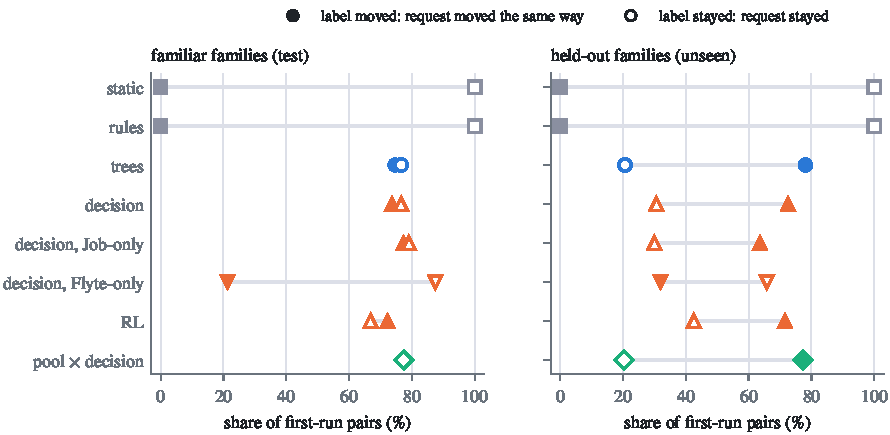
\includegraphics[width=\linewidth]{figures/fig_counterfactual.pdf}
\caption{The staging counterfactual, seed 1: the same first runs rendered as Jobs with the inputs on node disk and
on a memory-backed volume. Filled: among pairs whose label moved, the share where the request moved the same way.
Hollow: among pairs whose label stayed, the share where the request stayed too. Static requests and rules never
move on a first run.}
\label{fig:counterfactual}
\end{figure}

The models trained on Jobs read the manifest (\cref{fig:counterfactual,tab:cf}). When the label moves, the
decision model, the trees, RL and the pools move their request the right way on 72--78\% of familiar-code pairs and
64--78\% of unseen pairs. The Flyte-only model, which has never seen a manifest, does so on 21\%. Static requests and
rules never move, because on a first run they have only fixed defaults. On new code the models overreact: when the
label does not move, which mostly means the staged inputs were small, they still change their request on 57--80\% of
unseen pairs. They pick up the fetcher less reliably (31--47\% on test), which fits boto3's 48\,MiB only sometimes
crossing a cell.

\paragraph{The task's name.}
Generated tasks are named after their family (for example \code{pandas-join}), and the name appears in the code and
the manifest. We re-scored the counterfactual's first runs with each name replaced by a hash, without retraining
(\cref{tab:names}). On familiar code, regret changes by less than a point for every trained approach except the
Flyte-only model (+1.8); on new code it rises by 0.5--3.6 points. Each family also has a fixed function name and
input schema, which this test leaves in place, so it bounds the name's effect without removing the family's
identity from the code.

\subsection{The gate}
\label{sec:res-gate}

\Cref{tab:gate} compares the gate's signal with the alternatives. Correcting the first release's kNN scaling changed
nothing: the corrected distance still separates unseen families from validation with an AUROC of 0.999, sends every
unseen pod to RL, and gives exactly the same requests. The held-out families are far from the training data in code
tokens, though only one of them imports a library no training family uses (\cref{sec:dataset}). With code tokens
removed the AUROC falls to 0.67 and unseen regret rises to 66.4\%. The detector's job is easy on this
benchmark, and the benchmark cannot test it on new code built from familiar tokens.

\begin{table}[tbp]
\centering\small
\caption{Gate signals for seed 1. AUROC measures how well each signal ranks unseen pods above validation pods. The
middle columns give the share of pods routed to the RL model, and the last two the gate's regret on Job pods. All
gates use the 0.95 quantile except the disagreement gate, shown at 0.5.}
\label{tab:gate}
\begin{tabular}{@{}lrrrrr@{}}
\toprule
&& \multicolumn{2}{c}{sent to RL (\%)} & \multicolumn{2}{c}{Job regret (\%)} \\
\cmidrule(lr){3-4}\cmidrule(l){5-6}
signal & AUROC & test & unseen & test & unseen \\
\midrule
kNN, all features & 0.999 & 5.3 & 100.0 & 8.1\,{\scriptsize[7.0, 9.4]} & 39.3\,{\scriptsize[37.3, 41.3]} \\
kNN, k8s-1 scaling & 1.000 & 5.3 & 100.0 & 8.1\,{\scriptsize[7.0, 9.4]} & 39.3\,{\scriptsize[37.1, 41.4]} \\
kNN, numeric only & 0.673 & 4.5 & 30.5 & 7.9\,{\scriptsize[6.7, 9.2]} & 61.9\,{\scriptsize[59.0, 64.7]} \\
disagreement (JS), $q$ 0.5 & 0.729 & 51.3 & 80.5 & 11.5\,{\scriptsize[10.2, 13.0]} & 42.9\,{\scriptsize[40.8, 45.0]} \\
\bottomrule
\end{tabular}

\end{table}

Over three trainings, the gate averages \mTestGate\% on familiar code (\loTestGate--\hiTestGate\%) and
\mUnseenGate\% on new code (\loUnseenGate--\hiUnseenGate\%). Seed 3's familiar-code number is higher because its
familiar-code member, the pooled RL model read by argmax, was worse on that seed (17.5\%). On new code the gate always
equals the decoded RL model, whose temperature sits at its search bound (\cref{sec:methods}); validation would have
chosen that model's argmax read-out, which is about eight points worse on new code (\diffUnseenRLArgRL\ points
\diffUnseenRLArgRLCI).

\subsection{First runs and runs with history}
\label{sec:res-cold}

First runs are where the approaches differ most (\cref{tab:cold}). With history, most trained approaches do well on
familiar code (6--13\%), and rules-sized reaches 16.8\%. On first runs the rules lose most of their accuracy
(72--82\%), while the pooled decision model holds at 16.4\%. On new code, history does most of the work, and
rules-sized with history (16.9\%) is the best of any approach, because scaling the nearest earlier run by input size is a strong prior when a task's runs
differ only in size. Without history, no approach does well on new code; the best are the zero-shot model, on its
sample, and the gate.

\begin{table}[tbp]
\centering\small
\caption{Job regret (\%) on first runs and on runs with history, for seed 1.}
\label{tab:cold}
\begin{tabular}{@{}lrrrr@{}}
\toprule
& \multicolumn{2}{c}{test} & \multicolumn{2}{c}{unseen} \\
\cmidrule(lr){2-3}\cmidrule(l){4-5}
approach & first run & with history & first run & with history \\
\midrule
static & 107.7 & 90.4 & 137.4 & 106.2 \\
rules & 74.7 & 30.0 & 77.0 & 32.8 \\
rules-sized & 81.5 & 16.8 & 72.4 & \textbf{16.9} \\
zero-shot 27B & 98.0 & 24.6 & 59.6 & 36.1 \\
zero-shot 27B, JSON & 88.5 & 31.8 & 81.2 & 22.9 \\
trees & 22.0 & 12.9 & 115.5 & 37.6 \\
decision & 27.5 & 10.7 & 81.7 & 26.1 \\
RL, argmax & 23.2 & \textbf{6.2} & 80.5 & 24.6 \\
pool $\times$ decision & \textbf{16.4} & 8.2 & 103.9 & 23.8 \\
pool $\times$ RL, argmax & 19.3 & 7.4 & 145.9 & 30.6 \\
gate & 20.3 & 8.3 & \textbf{65.2} & 23.3 \\
\bottomrule
\end{tabular}

\end{table}

\subsection{Dollars and the price of a retry}
\label{sec:res-sens}

Mean regret counts every pod equally, while dollar regret is dominated by large jobs. On familiar code the two
mostly agree: the pooled RL model read by argmax costs \dTestPoolRLArg\% more than the cheapest requests in total,
and the gate \dTestGate\%. On new code, dollars rank the trees first (\dUnseenTrees\%), because they size the largest
jobs better even though their mean regret is among the worst. The trees cost \$\usdUnseenTrees{} per 1,000 unseen Job
runs, against \$\usdUnseenSized{} for rules-sized, \$\usdUnseenGate{} for the gate, and \$\usdCheapUnseen{} for the
cheapest requests.

A raw Job with \code{backoffLimit: 0} does not retry: it fails, and someone resubmits it. That makes an OOM much more
expensive than our default penalty. \Cref{fig:penalty,tab:sens} re-score every approach with penalties of 0, 5 and
20 times the label request's cost per retry. Every approach was tuned at the default penalty of 1, so this measures
how fixed requests hold up when failures get dearer, not how well each approach could adapt. On familiar code the
pooled decision model has the lowest regret at every penalty from 1 to 20 (\pTwentyTestPoolDec\% at 20), though at 20
the pooled RL model is within \sdTwentyTestPoolDecPoolRLArg{} points \sdTwentyTestPoolDecPoolRLArgCI. On new code,
rules-sized has the lowest regret at penalties of 5 and 20 (\pFiveUnseenSized\% and \pTwentyUnseenSized\%), ahead of RL
and the gate (\pFiveUnseenRL\% and \pTwentyUnseenGate\%). Clustered by task, that lead is clear
(\sdTwentyUnseenSizedGate\ points \sdTwentyUnseenSizedGateCI\ at 20); clustered by the seven families, it is not
(\sdFamTwentyUnseenSizedGateCI). For teams that run raw Jobs without retries, the evidence favours a rule that scales
by input size and reads the manifest on code nobody has seen before, and does not rule out the trained models.

\begin{figure}[tbp]
\centering
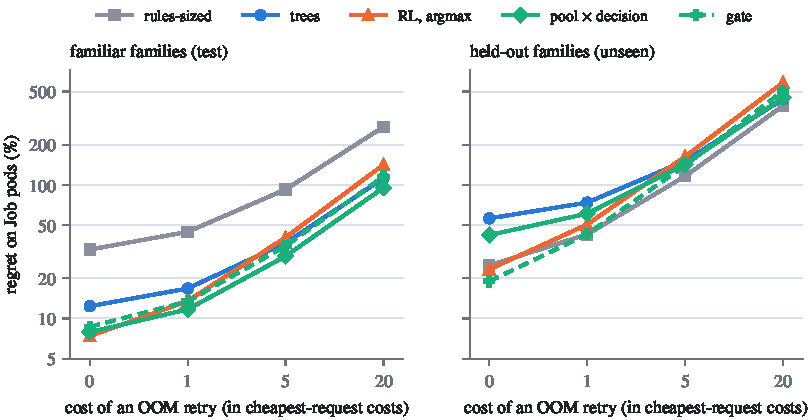
\includegraphics[width=\linewidth]{figures/fig_penalty.pdf}
\caption{Job regret as an OOM retry gets more expensive, seed 1 (log scale). Every approach was tuned at a penalty
of 1. On familiar code the trained approaches stay far ahead of rules-sized; on held-out families the lines cross,
and rules-sized has the lowest regret once a retry costs 5 or more.}
\label{fig:penalty}
\end{figure}

\begin{table}[tbp]
\centering\small
\caption{Job regret (\%) when each OOM retry costs 0, 1 (the default), 5 or 20 times the label request's cost.
Higher penalties stand for a Job that fails outright and has to be resubmitted.}
\label{tab:sens}
\resizebox{\linewidth}{!}{\begin{tabular}{@{}lrrrrrrrr@{}}
\toprule
& \multicolumn{2}{c}{0} & \multicolumn{2}{c}{1 (default)} & \multicolumn{2}{c}{5} & \multicolumn{2}{c}{20} \\
\cmidrule(lr){2-3}\cmidrule(lr){4-5}\cmidrule(lr){6-7}\cmidrule(l){8-9}
approach & test & unseen & test & unseen & test & unseen & test & unseen \\
\midrule
static & 47.8 & 44.3 & 89.3 & 115.1 & 255.2 & 398.2 & 877.6 & 1459.9 \\
rules & 28.8 & 24.7 & 42.4 & 49.8 & 96.9 & 149.9 & 301.2 & 525.6 \\
rules-sized & 25.9 & 20.9 & 37.7 & \textbf{39.2} & 84.9 & \textbf{112.5} & 261.8 & \textbf{387.2} \\
zero-shot 27B & 31.1 & 18.8 & 48.8 & 42.8 & 119.5 & 138.8 & 384.9 & 498.8 \\
zero-shot 27B, JSON & 26.5 & 24.4 & 48.8 & 44.4 & 138.0 & 124.4 & 472.6 & 424.4 \\
trees & 6.5 & 50.8 & 11.5 & 69.1 & 31.4 & 142.5 & 105.8 & 417.7 \\
decision & 7.3 & 20.2 & 12.6 & 47.8 & 33.8 & 158.6 & 113.3 & 573.8 \\
decision, argmax & 17.8 & 35.2 & 30.3 & 69.1 & 80.6 & 204.8 & 269.0 & 713.5 \\
RL & 8.1 & \textbf{15.2} & 14.6 & 39.3 & 40.4 & 135.7 & 137.3 & 497.1 \\
RL, argmax & \textbf{1.9} & 19.1 & 8.5 & 46.5 & 35.0 & 156.1 & 134.6 & 567.1 \\
pool $\times$ decision & 2.3 & 37.0 & \textbf{6.6} & 56.8 & \textbf{24.0} & 135.9 & \textbf{89.4} & 432.6 \\
pool $\times$ RL & 5.6 & 31.0 & 10.5 & 49.6 & 30.4 & 124.0 & 104.9 & 403.2 \\
pool $\times$ RL, argmax & 2.3 & 54.3 & 7.2 & 79.4 & 26.9 & 179.6 & 100.8 & 555.6 \\
gate (kNN, $q$ 0.95) & 2.9 & \textbf{15.2} & 8.1 & 39.3 & 29.1 & 135.7 & 107.7 & 497.1 \\
\bottomrule
\end{tabular}
}
\end{table}

\subsection{Three trainings}
\label{sec:res-seeds}

The static request, both rules and the trees give identical results on every seed. The trained models vary, more on
new code than on familiar code (\cref{tab:seeds}). On familiar code the top is stable: the pooled decision model ranges
from \loTestPoolDec\% to \hiTestPoolDec\% and RL read by argmax from \loTestRLArg\% to \hiTestRLArg\%. The pooled RL
model read by argmax ranges from \loTestPoolRLArg\% to \hiTestPoolRLArg\%. On new code, the decision model ranges from
\loUnseenDec\% to \hiUnseenDec\% and the pooled RL model read by argmax from \loUnseenPoolRLArg\% to
\hiUnseenPoolRLArg\%, while the gate varies least (\loUnseenGate--\hiUnseenGate\%). Rankings on new code within about
ten points of each other are not stable across trainings.

\begin{table}[tbp]
\centering\small
\caption{Job regret (\%) for each of the three trainings. The static request, the rules and the trees give identical
results on every seed.}
\label{tab:seeds}
\begin{tabular}{@{}lrrrrrr@{}}
\toprule
& \multicolumn{3}{c}{Job test, by seed} & \multicolumn{3}{c}{Job unseen, by seed} \\
\cmidrule(lr){2-4}\cmidrule(l){5-7}
approach & 1 & 2 & 3 & 1 & 2 & 3 \\
\midrule
static & 89.3 & 89.3 & 89.3 & 115.1 & 115.1 & 115.1 \\
rules & 42.4 & 42.4 & 42.4 & 49.8 & 49.8 & 49.8 \\
rules-sized & 37.7 & 37.7 & 37.7 & 39.2 & 39.2 & 39.2 \\
trees & 11.5 & 11.5 & 11.5 & 69.1 & 69.1 & 69.1 \\
decision & 12.6 & 13.4 & 15.0 & 47.8 & 44.2 & 56.6 \\
decision, argmax & 30.3 & 30.3 & 31.7 & 69.1 & 68.1 & 80.6 \\
RL & 14.6 & 16.7 & 17.4 & 39.3 & 38.2 & 35.5 \\
RL, argmax & 8.5 & 8.6 & 8.2 & 46.5 & 47.2 & 41.3 \\
pool $\times$ decision & 6.6 & 6.8 & 6.9 & 56.8 & 52.1 & 58.3 \\
pool $\times$ RL & 10.5 & 10.5 & 11.0 & 49.6 & 50.9 & 61.3 \\
pool $\times$ RL, argmax & 7.2 & 6.8 & 11.8 & 79.4 & 78.6 & 110.9 \\
gate (kNN, $q$ 0.95) & 8.1 & 8.1 & 12.7 & 39.3 & 38.2 & 35.5 \\
decision, Job-only & 13.2 & 13.8 & 12.2 & 56.1 & 53.3 & 68.5 \\
decision, Flyte-only & 37.3 & 33.8 & 37.5 & 59.0 & 67.1 & 76.1 \\
trees, Job-only & 11.8 & 11.8 & 11.8 & 68.6 & 68.6 & 68.6 \\
trees, Flyte-only & 18.3 & 18.3 & 18.3 & 73.5 & 73.5 & 73.5 \\
\bottomrule
\end{tabular}

\end{table}

\subsection{Zero-shot}
\label{sec:res-zs}

With room to finish its reasoning, the 27B model answers almost every prompt. \Cref{tab:zs} scores every approach on
the zero-shot model's own sample, so the comparison is like for like. On familiar code the zero-shot model
(\zsTestZS\%) is worse than the rules (\zsTestRules\% and \zsTestSized\%; paired difference with rules-sized
\diffTestZSSized\ points \diffTestZSSizedCI) and far behind the trained models (\zsTestRLArg\% for RL read by argmax). On
new code it is level with the best approaches on that sample (\zsUnseenZS\% against \zsUnseenSized\% for rules-sized and
\zsUnseenGate\% for the gate), with intervals of about $\pm$15 points. Constraining it to the JSON schema makes little
difference on Jobs and helps on Flyte tasks (\rFTestZSJ\% on familiar code).
